% Options for packages loaded elsewhere
\PassOptionsToPackage{unicode}{hyperref}
\PassOptionsToPackage{hyphens}{url}
\PassOptionsToPackage{dvipsnames,svgnames,x11names}{xcolor}
%
\documentclass[
  letterpaper,
  DIV=11,
  numbers=noendperiod]{scrartcl}

\usepackage{amsmath,amssymb}
\usepackage{iftex}
\ifPDFTeX
  \usepackage[T1]{fontenc}
  \usepackage[utf8]{inputenc}
  \usepackage{textcomp} % provide euro and other symbols
\else % if luatex or xetex
  \usepackage{unicode-math}
  \defaultfontfeatures{Scale=MatchLowercase}
  \defaultfontfeatures[\rmfamily]{Ligatures=TeX,Scale=1}
\fi
\usepackage{lmodern}
\ifPDFTeX\else  
    % xetex/luatex font selection
\fi
% Use upquote if available, for straight quotes in verbatim environments
\IfFileExists{upquote.sty}{\usepackage{upquote}}{}
\IfFileExists{microtype.sty}{% use microtype if available
  \usepackage[]{microtype}
  \UseMicrotypeSet[protrusion]{basicmath} % disable protrusion for tt fonts
}{}
\usepackage{xcolor}
\setlength{\emergencystretch}{3em} % prevent overfull lines
\setcounter{secnumdepth}{-\maxdimen} % remove section numbering
% Make \paragraph and \subparagraph free-standing
\ifx\paragraph\undefined\else
  \let\oldparagraph\paragraph
  \renewcommand{\paragraph}[1]{\oldparagraph{#1}\mbox{}}
\fi
\ifx\subparagraph\undefined\else
  \let\oldsubparagraph\subparagraph
  \renewcommand{\subparagraph}[1]{\oldsubparagraph{#1}\mbox{}}
\fi


\providecommand{\tightlist}{%
  \setlength{\itemsep}{0pt}\setlength{\parskip}{0pt}}\usepackage{longtable,booktabs,array}
\usepackage{calc} % for calculating minipage widths
% Correct order of tables after \paragraph or \subparagraph
\usepackage{etoolbox}
\makeatletter
\patchcmd\longtable{\par}{\if@noskipsec\mbox{}\fi\par}{}{}
\makeatother
% Allow footnotes in longtable head/foot
\IfFileExists{footnotehyper.sty}{\usepackage{footnotehyper}}{\usepackage{footnote}}
\makesavenoteenv{longtable}
\usepackage{graphicx}
\makeatletter
\def\maxwidth{\ifdim\Gin@nat@width>\linewidth\linewidth\else\Gin@nat@width\fi}
\def\maxheight{\ifdim\Gin@nat@height>\textheight\textheight\else\Gin@nat@height\fi}
\makeatother
% Scale images if necessary, so that they will not overflow the page
% margins by default, and it is still possible to overwrite the defaults
% using explicit options in \includegraphics[width, height, ...]{}
\setkeys{Gin}{width=\maxwidth,height=\maxheight,keepaspectratio}
% Set default figure placement to htbp
\makeatletter
\def\fps@figure{htbp}
\makeatother
\newlength{\cslhangindent}
\setlength{\cslhangindent}{1.5em}
\newlength{\csllabelwidth}
\setlength{\csllabelwidth}{3em}
\newlength{\cslentryspacingunit} % times entry-spacing
\setlength{\cslentryspacingunit}{\parskip}
\newenvironment{CSLReferences}[2] % #1 hanging-ident, #2 entry spacing
 {% don't indent paragraphs
  \setlength{\parindent}{0pt}
  % turn on hanging indent if param 1 is 1
  \ifodd #1
  \let\oldpar\par
  \def\par{\hangindent=\cslhangindent\oldpar}
  \fi
  % set entry spacing
  \setlength{\parskip}{#2\cslentryspacingunit}
 }%
 {}
\usepackage{calc}
\newcommand{\CSLBlock}[1]{#1\hfill\break}
\newcommand{\CSLLeftMargin}[1]{\parbox[t]{\csllabelwidth}{#1}}
\newcommand{\CSLRightInline}[1]{\parbox[t]{\linewidth - \csllabelwidth}{#1}\break}
\newcommand{\CSLIndent}[1]{\hspace{\cslhangindent}#1}

%\documentclass{article}

% todonotes package                          #####################

\usepackage[textsize=footnotesize]{todonotes}


%language                                    #####################

%\usepackage{times}
%\usepackage{t1enc}                               Trouble maker
%\usepackage[utf8x]{inputenc}
%\usepackage[polish]{babel}
%\usepackage{polski}


% math                                       #####################

%AMS
\usepackage{amsfonts}
%\usepackage{amssymb}
%\usepackage{amsthm}
\usepackage{amsmath}
\usepackage{mathtools}


% page geometry                              #####################


\usepackage{geometry}
 \geometry{a4paper,left=35mm,top=20mm,}

\setlength{\parindent}{10pt}
\setlength{\parskip}{1pt}

\usepackage{float}


% abbreviations                              #####################

\newcommand{\ra}{\rangle}
\newcommand{\la}{\langle}
\newcommand{\n}{\neg}
\newcommand{\et}{\wedge}
\newcommand{\jt}{\rightarrow}
\newcommand{\ko}[1]{\forall  #1\,}
\newcommand{\ro}{\leftrightarrow}
\newcommand{\exi}[1]{\exists\, {_{#1}}}
\newcommand{\pr}[1]{\mathsf{P}(#1)}
\newcommand{\cost}{\mathsf{cost}}
\newcommand{\benefit}{\mathsf{benefit}}
\newcommand{\ut}{\mathsf{ut}}

\newcommand{\odds}{\mathsf{Odds}}
\newcommand{\ind}{\mathsf{Ind}}
\newcommand{\nf}[2]{\nicefrac{#1\,}{#2}}
\newcommand{\R}[1]{\texttt{#1}}
\newcommand{\prr}[1]{\mbox{$\mathtt{P}_{prior}(#1)$}}
\newcommand{\prp}[1]{\mbox{$\mathtt{P}_{posterior}(#1)$}}

\newcommand{\s}[1]{\mbox{$\mathsf{#1}$}}


\newtheorem{q}{\color{blue}Question}
\newtheorem{lemma}{Lemma}
\newtheorem{theorem}{Theorem}



% bibliography                                #####################

\usepackage[authoryear]{natbib}

%\bibliographystyle{apalike}





\KOMAoption{captions}{tableheading}
\makeatletter
\makeatother
\makeatletter
\makeatother
\makeatletter
\@ifpackageloaded{caption}{}{\usepackage{caption}}
\AtBeginDocument{%
\ifdefined\contentsname
  \renewcommand*\contentsname{Table of contents}
\else
  \newcommand\contentsname{Table of contents}
\fi
\ifdefined\listfigurename
  \renewcommand*\listfigurename{List of Figures}
\else
  \newcommand\listfigurename{List of Figures}
\fi
\ifdefined\listtablename
  \renewcommand*\listtablename{List of Tables}
\else
  \newcommand\listtablename{List of Tables}
\fi
\ifdefined\figurename
  \renewcommand*\figurename{Figure}
\else
  \newcommand\figurename{Figure}
\fi
\ifdefined\tablename
  \renewcommand*\tablename{Table}
\else
  \newcommand\tablename{Table}
\fi
}
\@ifpackageloaded{float}{}{\usepackage{float}}
\floatstyle{ruled}
\@ifundefined{c@chapter}{\newfloat{codelisting}{h}{lop}}{\newfloat{codelisting}{h}{lop}[chapter]}
\floatname{codelisting}{Listing}
\newcommand*\listoflistings{\listof{codelisting}{List of Listings}}
\makeatother
\makeatletter
\@ifpackageloaded{caption}{}{\usepackage{caption}}
\@ifpackageloaded{subcaption}{}{\usepackage{subcaption}}
\makeatother
\makeatletter
\@ifpackageloaded{tcolorbox}{}{\usepackage[skins,breakable]{tcolorbox}}
\makeatother
\makeatletter
\@ifundefined{shadecolor}{\definecolor{shadecolor}{rgb}{.97, .97, .97}}
\makeatother
\makeatletter
\makeatother
\makeatletter
\makeatother
\ifLuaTeX
  \usepackage{selnolig}  % disable illegal ligatures
\fi
\IfFileExists{bookmark.sty}{\usepackage{bookmark}}{\usepackage{hyperref}}
\IfFileExists{xurl.sty}{\usepackage{xurl}}{} % add URL line breaks if available
\urlstyle{same} % disable monospaced font for URLs
\hypersetup{
  pdftitle={Second-order Probabilism: Expressive Power and Accuracy},
  pdfauthor={Rafal Urbaniak and Marcello Di Bello},
  colorlinks=true,
  linkcolor={blue},
  filecolor={Maroon},
  citecolor={Blue},
  urlcolor={Blue},
  pdfcreator={LaTeX via pandoc}}

\title{Second-order Probabilism: Expressive Power and Accuracy}
\author{Rafal Urbaniak and Marcello Di Bello}
\date{2023-09-06}

\begin{document}
\maketitle
\ifdefined\Shaded\renewenvironment{Shaded}{\begin{tcolorbox}[frame hidden, interior hidden, borderline west={3pt}{0pt}{shadecolor}, boxrule=0pt, enhanced, sharp corners, breakable]}{\end{tcolorbox}}\fi

\renewcommand*\contentsname{Table of contents}
{
\hypersetup{linkcolor=}
\setcounter{tocdepth}{3}
\tableofcontents
}
\vspace{2cm}

\noindent \textbf{DISCLAIMER:}
\textbf{This is a draft of work in progress, please do not cite or distribute without permission.}

\thispagestyle{empty}

\newpage

\begin{quote} \textbf{Abstract.}  \todo{need to write one when done}

\end{quote}

\hypertarget{introduction}{%
\section{Introduction}\label{introduction}}

\label{sec:introduction}

Precise probabilism (PP) has it that a rational agent's (RA) uncertainty
is to be represented as a single probability measure. The view has been
criticized on the ground that RA's degrees of belief are not
appropriately evidence-responsive, especially when evidence is scant.
Accordingly, an alternative view---imprecise probabilism (IP)---has been
proposed, on which RA's uncertainty is to be represented by a set of
probability measures, rather than a unique one.

Unfortunately, this view runs into problems as well. (1) It still does
not seem to be sufficiently evidence-responsive, (2) it is claimed to
get certain comparative probability judgments wrong, (3) it seems to be
unable to model learning when the starting point is complete lack of
information, and (4) notoriously there exist no inaccuracy measure of an
imprecise credal stance if the measure is to satisfy certain
straightforward formal conditions.

\todo{Think about including synergy}

The main claim of this paper is that the way forward is to use
higher-order probabilities to represen't RA's uncertainty in the
relevant cases. The key idea is that uncertainty is not a
single-dimensional thing to be mapped on a single one-dimensional scale
like a real line and that it's the whole shape of the whole distribution
over parameter values that should be taken under consideration. This
guiding idea can be used to resolve many problems and philosophical
puzzles raised in the debate between PP and IP. Moreover, Bayesian
probabilistic programming already provides a fairly reliable
implementation framework of this approach.

\todo{add structure description}

\hypertarget{precise-vs.-imprecise-probabilisms}{%
\section{Precise vs.~imprecise
probabilisms}\label{precise-vs.-imprecise-probabilisms}}

\label{sec:three-probabilism}

\hypertarget{precise-probabilism}{%
\subsection{Precise probabilism}\label{precise-probabilism}}

Precise probabilism (\textsf{PP}) holds that a rational agent's
uncertainty about a hypothesis is to be represented as a single, precise
probability measure. This is an elegant and simple theory. But
representing our uncertainty about a proposition in terms of a single,
precise probability runs into a number of difficulties. Precise
probabilism---arguably---fails to capture an important dimension of how
our fallible beliefs reflect the evidence we have (or have not)
obtained. A couple of stylized examples should make the point clear. For
the sake of simplicity, we will use examples featuring coins.

\begin{quote}
\textbf{No evidence v. fair coin}
You are about to toss a coin, but have no evidence 
whatsoever about its bias. You are completely ignorant. 
Compare this to the situation in which you know, 
based on overwhelming evidence, that the coin is fair. 
\end{quote}

\noindent On precise probabilism, both scenarios are represented by
assigning a probability of .5 to the outcome \emph{heads}. If you are
completely ignorant, the principle of insufficient evidence suggests
that you assign .5 to both outcomes. Similarly, if you know for sure the
coin is fair, assigning .5 seems the best way to quantify the
uncertainty about the outcome. The agent's evidence in the two scenario
is quite different, but precise probabilities fail to capture this
difference.

\begin{quote}
\textbf{Learning from ignorance}
You toss a coin with unknown bias. You toss it 10 times and observe \emph{heads} 5 times. Suppose you toss it further and observe 50 \emph{heads} in 100 tosses. 
\end{quote}

\noindent Since the coin initially had unknown bias, you should
presumably assign a probability of .5 to both outcomes if you stick with
\textsf{PP}. After the 10 tosses, you end up again with an estimate of
.5. You must have learned something, but whatever that is, it is not
modeled by precise probabilities. When you toss the coin 100 times and
observe 50 heads, you learn something new as well. But your precise
probability assessment will again be .5.

These examples suggest that precise probabilism is not appropriately
responsive to evidence when it comes to representing what RA justifiedly
believes of has learned. It ends up assigning the same probability in
situations in which one's evidence is quite different: when no evidence
is available about the coin's bias; when there is little evidence that
the coin is fair (say, after only 10 tosses); and when there is strong
evidence that the coin is fair (say, after 100 tosses). The general
problem is, precise probability captures the value around which your
uncertainty should be centered, but fails to capture how centered it
should be given the evidence.\footnote{In fact, analogous problems arise
  even if we do not start with complete lack of evidence; if RA
  initially weakly believes that the coin is .6 biased towards heads, as
  she might still learn more, by confirming her belief by tossing the
  coin repeatedly and observing, say, 60 heads in 100 tosses---but this
  improvement is not mirrored in the precise probability she will assign
  to heads.}

Precise probabilism, it has been argued, fails also to account for cases
in which an agent remains undecided even after some additional evidence
has been obtained. Imagine RA doesn't know what the bias of the coin is,
which PP represents as \(\pr(H)= .5\). Then she learns that the bias
towards heads has been slightly increased by .001 (in the philosophical
literature, this is called \emph{sweetening}. Intuitively, this might
still leave RA equally undecided when it comes to betting on \(H\). that
would've been fair even if the actual chance of \(H\) was .5 and not
.001. The same sweetening, however, should make RA bet on \(H\) if their
original lack of information was in fact correctly captured as a precise
credence.

\hypertarget{imprecise-probabilism}{%
\subsection{Imprecise probabilism}\label{imprecise-probabilism}}

What if we give up the assumption that probability assignments should be
precise? Imprecise probabilism (\textsf{IP}) holds that an agent's
credal stance towards a hypothesis is to be represented by means of a
\emph{set of probability measures}, typically called a representor
\(\mathbb{P}\), rather than a single measure \(\mathsf{P}\). The
representor should include all and only those probability measures which
are compatible with the evidence. For instance, if an agent knows that
the coin is fair, their credal state would be represented by the
singleton set \(\{\mathsf{P}\}\), where \(\mathsf{P}\) is a probability
measure which assigns \(.5\) to \emph{heads}. If, on the other hand, the
agent knows nothing about the coin's bias, their credal state would be
represented by the set of all probabilistic measures, since none of them
is excluded by the available evidence. Note that the set of probability
measures does not represent admissible options that the agent could
legitimately pick from. Rather, the agent's credal state is essentially
imprecise and should be represented by means of the entire set of
probability measures.\footnote{For the development of imprecise
  probabilism, see Keynes (1921); Levi (1974); Gärdenfors \& Sahlin
  (1982); Kaplan (1968); Joyce (2005); Fraassen (2006); Sturgeon (2008);
  Walley (1991). Bradley (2019) is a good source of further references.
  Imprecise probabilism shares some similarities with what we might call
  \textbf{interval probabilism} (Kyburg, 1961;
  \textbf{kyburg2001uncertain?}). On interval probabilism, precise
  probabilities are replaced by intervals of probabilities. On imprecise
  probabilism, instead, precise probabilities are replaced by sets of
  probabilities. This makes imprecise probabilism more general, since
  the probabilities of a proposition in the representor set do not have
  to form a closed interval. In what follows, we will ignore interval
  probabilism, as intervals do not contain probabilistic information
  sufficient to guide reasoning with multiple items of evidence.}

Imprecise probabilism, at least \emph{prima facie}, offers a
straightforward picture of learning from evidence, that is a natural
extension of the classical Bayesian approach. When faced with new
evidence \(E\) between time \(t_0\) and \(t_1\), the representor set
should be updated point-wise, running the standard Bayesian updating on
each probability measure in the representor:

\begin{align*}
\mathbb{P}_{t_1} = \{\mathsf{P}_{t_1}\vert \exists\, {\mathsf{P}_{t_0} \!\in  \mathbb{P}_{t_0}}\,\, \forall\, {H}\,\, \left[\mathsf{P}_{t_1}(H)=\mathsf{P}_{t_0}(H \vert E)\right] \}.
\end{align*} \label{eq:updateRepresentor}

\noindent The hope is that, if we start with a range of probabilities
that is not extremely wide, point-wise learning will behave
appropriately. For instance, if we start with a prior probability of
\emph{heads} equal to .4 or .6, then those measure should be updated to
something closer to \(.5\) once we learn that a given coin has already
been tossed ten times with the observed number of heads equal 5 (call
this evidence \(E\)). This would mean that if the initial range of
values was \([.4,.6]\) the posterior range of values should be more
narrow.

But even this seemingly straightforward piece of reasoning is hard to
model without using densities. For to calculate
\(\pr{\s{bias} = k \vert E}\) we need to calculate
\(\pr{E \vert \s{bias} = k }\pr{\s{bias} = k}\) and divide it by
\(\pr{E} = \pr{E \vert \s{bias} = k }\pr{\s{bias = k}} + \pr{E \vert \s{bias} \neq k }\pr{ \s{bias} \neq k}\).
The tricky part is obtaining \(\pr{\s{bias} = k}\) or
\(\pr{ \s{bias} \neq k}\) in a principled manner without explicitly
going second-order, without estimating the parameter value and without
using beta distributions.

The situation is even more difficult if we start with complete lack of
knowledge, as imprecise probabilism runs into the problem of
\textbf{belief inertia} (Levi, 1980). Say you start tossing a coin
knowing nothing about its bias. The range of possibilities is \([0,1]\).
After a few tosses, if you observed at least one tail and one heads, you
can exclude the measures assigning 0 or 1 to \emph{heads}. But what else
have you learned? If you are to update your representor set point-wise,
you will end up with the same representor set. Consequently, the edges
of your resulting interval will remain the same. In the end, it is not
clear how you are supposed to learn anything if you start from complete
ignorance.

Here's another example from Rinard (2013). Either all the marbles in the
urn are green (\(H_1\)), or exactly one tenth of the marbles are green
(\(H_2\)). Your initial credence is complete uncertainty with interval
\([0,1]\) associated with each hypothesis. Then you learn that a marble
drawn at random from the urn is green (\(E\)). After conditionalizing
each function in your representor on this evidence, you end up with the
the same spread of values for \(H_1\) that you had before learning
\(E\), and no matter how many marbles are sampled from the urn and found
to be green.

Some downplay the problem of belief inertia. They insist that vacuous
priors should not be used and that imprecise probabilism gives the right
results when the priors are non-vacuous. After all, if you started with
knowing truly nothing, then perhaps it is right to conclude that you
will never learn anything. Another strategy is to say that, in a state
of complete ignorance, a special updating rule should be
deployed.\footnote{Lee (2017) suggests the rule of
  \emph{credal set replacement} that recommends that upon receiving
  evidence the agent should drop measures rendered implausible, and add
  all non-extreme plausible probability measures. This, however, is
  tricky. One needs a separate account of what makes a distribution
  plausible or not, as well as a principled account of why one should
  use a separate special update rule when starting with complete
  ignorance.} But no matter what we think about belief inertia, other
problems plague imprecise probabilism. Three problems are particularly
pressing.

One problem is that \textbf{imprecise probabilism fails to capture
intuitions we have about evidence and uncertainty in a number of
scenarios.} Consider this example:

\begin{quote}
\textbf{Even v. uneven bias:}
 You have two coins and you know, for sure, that the probability of getting heads is .4, if you toss one coin, and .6, if you toss the other coin. But you do not know which is which. You pick one of the two at random and toss it.  Contrast this with an uneven case. You have four coins and you know that three of them have bias $.4$ and one of them has bias $.6$. You pick a coin at random and plan to toss it. You should be three times more confident that the probability of getting heads is .4. rather than .6.
\end{quote}

\noindent The first situation can be easily represented by imprecise
probabilism. The representor would contain two probability measures, one
that assigns .4. and the other that assigns .6 to the hypothesis `this
coin lands heads'. But imprecise probabilism cannot represent the second
situation, at least not without moving to higher-order probabilities or
assigning probabilities to chance hypotheses, in which case it is no
longer clear whether the object-level imprecision does any heavy
lifting.\footnote{Other scenarios can be constructed in which imprecise
  probabilism fails to capture distinctive intuitions about evidence and
  uncertainty; see, for example, (Rinard, 2013). Suppose you know of two
  urns, \textsf{GREEN} and \textsf{MYSTERY}. You are certain
  \textsf{GREEN} contains only green marbles, but have no information
  about \textsf{MYSTERY}. A marble will be drawn at random from each.
  You should be certain that the marble drawn from \textsf{GREEN} will
  be green (\(G\)), and you should be more confident about this than
  about the proposition that the marble from \textsf{MYSTERY} will be
  green (\(M\)). In line with how lack of information is to be
  represented on \textsf{IP}, for each \(r\in [0,1]\) your representor
  contains a \(\mathsf{P}\) with \(\pr{M}=r\). But then, it also
  contains one with \(\pr{M}=1\). This means that it is not the case
  that for any probability measure \(\mathsf{P}\) in your representor,
  \(\mathsf{P}(G) > \mathsf{P}(M)\), that is, it is not the case that RA
  is more confident of \(G\) than of \(M\). This is highly
  counter-intuitive.}

Second, besides descriptive inadequacy, imprecise probabilism fases a
foundational problem. It arises when we attempt to measure the accuracy
of a representor set of probability measures. Workable \emph{scoring
rules} exist for measuring the accuracy of a single, precise credence
function, such as the Brier score. These rules measure the distance
between one's credence function (or probability measure) and the actual
value. A requirement of scoring rules is that they be \emph{proper}: any
agent will score their own credence function to be more accurate than
every other credence function. After all, if an agent thought a
different credence was more accurate, they should switch to it. Proper
scoring rules are then used to formulate accuracy-based arguments for
precise probabilism. These arguments show (roughly) that, if your
precise credence follows the axioms of probability theory, no other
credence is going to be more accurate than yours whatever the facts are.
Can the same be done for imprecise probabilism? It seems not.
Impossibility theorems demonstrate that \textbf{no proper scoring rules
are available for representor sets}. So, as many have noted, the
prospects for an accuracy-based argument for imprecise probabilism look
dim (Campbell-Moore, 2020; Mayo-Wilson \& Wheeler, 2016; Schoenfield,
2017; Seidenfeld, Schervish, \& Kadane, 2012). Moreover, as shown by
Schoenfield (2017), if an accuracy measure satisfies certain plausible
formal constraints, it will never strictly recommend an imprecise
stance, as for any imprecise stance there will be a precise one with at
least the same accuracy.

The third problem with imprecise probabilism is that, \textbf{degenerate
cases aside, it is hard to make sense of the notion of an IP agent
learning that a probabilistic measure is incompatible with the
evidence.} Recall that the probability measures allowed in a representor
set are supposed to be only those compatible with the agent's evidence.
The idea is that thanks to this feature, imprecise credal stances are
evidence-responsive in a way precise probabilistic stances are not. But
how, exactly, does the evidence exclude probability measures?

This is not a mathematical question: mathematically
(\textbf{bradley2012scientific?}), evidential constraints are easy to
model. They can take the form, for example, of the
\emph{evidence of chances} \(\{ \mathsf{P}(X) = x\}\) or
\(\mathsf{P}(X) \in [x,y]\), or \emph{structural constraints} such as
``\(X\) and \(Y\) are independent'' or ``\(X\) is more likely than
\(Y\).'' While it is clear that these constraints are something that an
agent can come to accept if offered such information by an expert to
which the agent completely defers, it is not trivial to explain how
non-testimonial evidence can result in such constraints for an epistemic
agent that functions as IP proposes.

Most of the examples in the literature start with the assumption that
the agent is told by a believable source that the chances are
such-and-such, or that the experimental set-up is such that the agent
knows that such and such structural constraint is satisfied. But,
besides ideal circumstances, it is unclear how an agent could come to
accept such structural constraints upon observation. The chain of
testimonial evidence has to end somewhere.

Admittedly, there are straightforward degenerate cases: if you see the
outcome of a coin toss to be heads, you reject the measure with
\(\mathsf{P}(H)=0\), and similarly for tails. Another class of cases
might arise if you are randomly drawing objects from a finite set where
the real frequencies are already known, because this finite set has been
inspected. But such extreme cases aside, what else? Mere consistency
constraint wouldn't get the agent very far in the game of excluding
probability measures, as way too many probability measures are strictly
speaking still consistent with the observations for evidence to result
in epistemic progress.\^{}{[} Bradley suggests that ``statistical
evidence might inform {[}evidential{]} constraints {[}\dots and that
evidence{]} of causes might inform structural constraints''
{[}125-126{]}. This, however, is not a clear account of how exactly this
should proceed. One suggestion might be that once a statistical
significance threshold is selected, a given set of observations with a
selection of background modeling assumptions yields a credible interval.
But this is to admit that to reach such constraints, we already have to
start with a second-order approach, and drop information about the
densities, focusing only on the intervals obtained with fixed margins of
errors. But as we will be insisting, if you have the information about
densities to start with, there is no clear advantage to going imprecise
instead, and there are multiple problems associated with this move.
Moreover, such moves require a choice of an error margin, which is
extra-epistemic, and it is not clear what advantage there is to use
extra-epistemic considerations of this sort to drop information
contained in densities.\footnote{Relatedly, in forensic evidence
  evaluation even scholars who disagree about the value of going
  higher-order agree that interval reporting is problematic, as the
  choice of a limit or uncertainty level is rather arbitrary
  (\textbf{Taroni2015Dismissal?}; \textbf{Sjerps2015Uncertainty?}).}

\hypertarget{higher-order-probabilism}{%
\subsection{Higher-order probabilism}\label{higher-order-probabilism}}

There is, however, a view in the neighborhood that fares better: a
higher-order perspective. In fact, some of the comments by the
proponents of imprecise probabilism tend to go in this direction. For
instance, Bradley compares the measures in a representor to committee
members, each voting on a particular issue, say the true bias of a coin.
As they acquire more evidence, the committee members will often converge
on a specific chance hypothesis. He writes
(\textbf{bradley2012scientific?}):

\begin{quote}
\dots the committee members are ''bunching up''. Whatever measure you put over the set of probability functions---whatever ''second order probability'' you use---the ''mass'' of this measure gets more and more concentrated around the true chance hypothesis'.
\end{quote}

\noindent Note, however, that such bunching up cannot be modeled by
imprecise probabilism alone.\footnote{Bradley seems to be aware of that,
  which would explain the use of scare quotes: when he talks about the
  option of using second-order probabilities in decision theory, he
  insists that `there is no justification for saying that there is more
  of your representor here or there.'
  \textasciitilde{[}p.\textasciitilde195{]}}

In a similar vein, Joyce (2005), in a paper defending imprecise
probabilism, attempts to explicate something that imprecise probabilism
was advertised to handle better than precise probabilism: weight of
evidence. But in fact, the explication uses a density over chance
hypotheses to account for the notion of evidential weight and
conceptualizes the weight of evidence as an increase of concentration of
smaller subsets of chance hypotheses, without any reference to
representors in the explication of the notion of weight.

\#(we will get back to his explication when we discuss weight of
evidence).

The idea that one should use higher-order probabilities has also been
suggested by critics of imprecise probabilism. For example, Carr (2020)
argues that sometimes evidence requires uncertainty about what credences
to have. Carr, however, does not articulate this suggestion more fully,
does not develop it formally, and does not explain how her approach
would fare against the difficulties affecting precise ad imprecise
probabilism. This is the key goal of this paper.

The underlying idea of the higher-order approach we propose is that
\textbf{uncertainty is not a single-dimensional thing to be mapped on a
single one-dimensional scale such as a real line. It is the whole shape
of the whole distribution over parameter values that should be taken
under consideration.}\footnote{Bradley admits this much
  (\textbf{bradley2012scientific?}), and so does Konek (Konek, 2013, p.
  59). For instance, Konek disagrees with: (1) \(X\) is more probable
  than \(Y\) just in case \(p(X)>p(Y)\), (2) \(D\) positively supports
  \(H\) if \(p_D(H)> p(H)\), or (3) \(A\) is preferable to \(B\) just in
  case the expected utility of \(A\) w.r.t. \(p\) is larger than that of
  \(B\).} From this perspective, when an agent is asked about their
credal stance towards \(X\), they can refuse to summarize it in terms of
a point value \(\mathsf{P}(X)\). They can instead express their credal
stance in terms of a probability (density) distribution \(f_x\) treating
\(\mathsf{P}(X)\) as a random variable. To be sure, an agent's credal
state toward \(X\) could sometimes be usefully represented by the
expectation, especially when the agent is quite confident about the
probability of a given proposition.

Generally, expectation is defined as \(\int_{0}^{1} x f(x) \, dx\)--in
the context of our approach here, we can think of \(x\) as the
objectively appropriate/justified degree of belief in a given
proposition, and of \(f\) as the density representing the agent's
uncertainty about \(x\). Perhaps, such an expectation can be used as the
precise, object-level credence in the proposition itself, where \(f\) is
the probability density over possible object-level probability values.
But this need not always be the case. If the probability density \(f\)
is not sufficiently concentrated around a single value, a one-point
summary might fail to do justice to the nuances of the agent's credal
state. This approach lines up with common practice in Bayesian
statistics, where the primary role of uncertainty representation is
assigned to the whole distribution. Summaries such as the mean, mode
standard deviation, mean absolute deviation, or highest posterior
density intervals are only succinct ways for representing the
uncertainty of a given scenario.

For example, consider again the scenario in which the agent knows that
the bias of the coin is either .4 or .6 but the former is three times
more likely. Representing the agent's credal state with the expectation
\(\mathsf{P}(X) = .75 \times .4 + .25 \times .6 = .45\) would fail to
capture an important feature of RA's belief---that she believes the two
biases to be of hugely different plausibilities, and that she in fact is
certain that the bias is \emph{not} .75.

This higher-order approach as a technical devise is not very surprising.
Bayesian probabilistic programming languages embrace the well-known idea
that parameters can be stacked and depend on each other in more or less
complicated manners.\todo{Cite PP without tears here} What is however
surprising is that while the technical devise has been available, it
hasn't been implemented to model agent's uncertainty, and by the same
token to address all the challenging scenarios we discussed so far.

Once we allow more expressive power in this fashion, we obtain rather
straightforwardly obtain more honest representations of RA's credal
states, illustrated in Figure \ref{fig-evidenceResponse}. In particular,
the scenario in which the two biases of the coin are not equally
likely---which imprecise probabilism cannot model---can be easily
modeled within high-order probabilism by assigning different
probabilities to the two biases.

\begin{figure}

{\centering 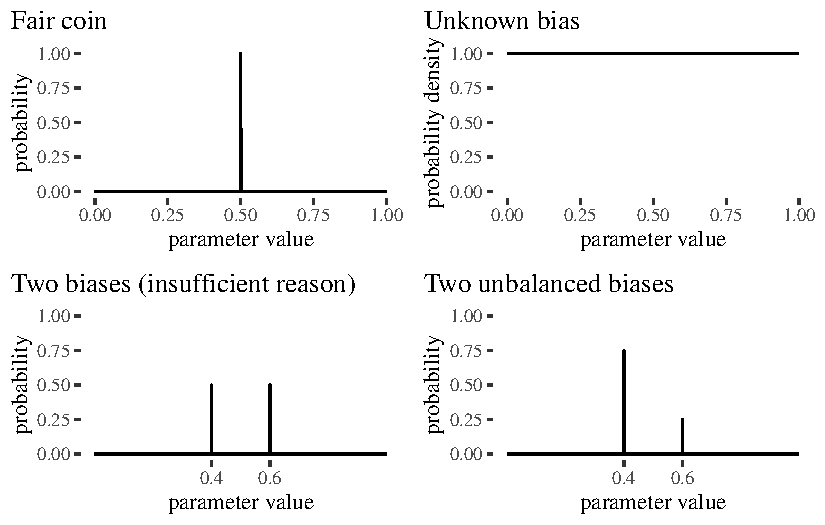
\includegraphics[width=0.8\textwidth,height=\textheight]{imp_MWE_files/figure-pdf/fig-evidenceResponse-1.pdf}

}

\caption{\label{fig-evidenceResponse}Examples of higher-order
distributions for a few scenarios problematic for both precise and
imprecise probabilism.}

\end{figure}

Let's try this figure \ref{fig-evidenceResponse}.

\begin{figure}


::: {.cell}

```{.r .cell-code}
grid.arrange(FairPlot,UniformPlot, TwoPlot, TwoUnbalancedPlot)
```

::: {.cell-output-display}
![](imp_MWE_files/figure-pdf/unnamed-chunk-1-1.pdf){fig-pos='H'}
:::
:::


\label{fig-theFigure}
\caption{caption of the figure}
\end{figure}

\hypertarget{refs}{}
\begin{CSLReferences}{1}{0}
\leavevmode\vadjust pre{\hypertarget{ref-bradley2019imprecise}{}}%
Bradley, S. (2019). {Imprecise Probabilities}. In E. N. Zalta (Ed.),
\emph{The {Stanford} encyclopedia of philosophy} ({S}pring 2019).
\url{https://plato.stanford.edu/archives/spr2019/entries/imprecise-probabilities/};
Metaphysics Research Lab, Stanford University.

\leavevmode\vadjust pre{\hypertarget{ref-CampbellMoore2020accuracy}{}}%
Campbell-Moore, C. (2020). \emph{Accuracy and imprecise probabilities}.

\leavevmode\vadjust pre{\hypertarget{ref-Carr2020impreciseEvidence}{}}%
Carr, J. R. (2020). Imprecise evidence without imprecise credences.
\emph{Philosophical Studies}, \emph{177}(9), 2735--2758.
\url{https://doi.org/10.1007/s11098-019-01336-7}

\leavevmode\vadjust pre{\hypertarget{ref-VanFraassen2006vague}{}}%
Fraassen, B. C. V. (2006). Vague expectation value loss.
\emph{Philosophical Studies}, \emph{127}(3), 483--491.
\url{https://doi.org/10.1007/s11098-004-7821-2}

\leavevmode\vadjust pre{\hypertarget{ref-Gardenfors1982unreliable}{}}%
Gärdenfors, P., \& Sahlin, N.-E. (1982). Unreliable probabilities, risk
taking, and decision making. \emph{Synthese}, \emph{53}(3), 361--386.
\url{https://doi.org/10.1007/bf00486156}

\leavevmode\vadjust pre{\hypertarget{ref-joyce2005probabilities}{}}%
Joyce, J. M. (2005). How probabilities reflect evidence.
\emph{Philosophical Perspectives}, \emph{19}(1), 153--178.

\leavevmode\vadjust pre{\hypertarget{ref-Kaplan1968decision}{}}%
Kaplan, J. (1968). Decision theory and the fact-finding process.
\emph{Stanford Law Review}, \emph{20}(6), 1065--1092.

\leavevmode\vadjust pre{\hypertarget{ref-keynes1921treatise}{}}%
Keynes, J. M. (1921). \emph{A treatise on probability, 1921}. London:
Macmillan.

\leavevmode\vadjust pre{\hypertarget{ref-konek2013foundations}{}}%
Konek, J. (2013). \emph{New foundations for imprecise bayesianism} (PhD
thesis). University of Michigan.

\leavevmode\vadjust pre{\hypertarget{ref-Kyburg1961}{}}%
Kyburg, H. E. (1961). \emph{Probability and the logic of rational
belief}. Wesleyan University Press.

\leavevmode\vadjust pre{\hypertarget{ref-Lee2017impreciseEpistemology}{}}%
Lee, E. (2017). \emph{Imprecise probability in epistemology} (PhD
thesis). Ludwig-Maximilians-Universit{ä}t;
Ludwig-Maximilians-Universität München.

\leavevmode\vadjust pre{\hypertarget{ref-Levi1974ideterminate}{}}%
Levi, I. (1974). On indeterminate probabilities. \emph{The Journal of
Philosophy}, \emph{71}(13), 391. \url{https://doi.org/10.2307/2025161}

\leavevmode\vadjust pre{\hypertarget{ref-Levi1980enterprise}{}}%
Levi, I. (1980). \emph{The enterprise of knowledge: An essay on
knowledge, credal probability, and chance}. MIT Press.

\leavevmode\vadjust pre{\hypertarget{ref-Mayo-Wilson2016scoring}{}}%
Mayo-Wilson, C., \& Wheeler, G. (2016). Scoring imprecise credences: A
mildly immodest proposal. \emph{Philosophy and Phenomenological
Research}, \emph{92}(1), 55--78.
\url{https://doi.org/10.1111/phpr.12256}

\leavevmode\vadjust pre{\hypertarget{ref-Rinard2013against}{}}%
Rinard, S. (2013). Against radical credal imprecision. \emph{Thought: A
Journal of Philosophy}, \emph{2}(1), 157--165.
\url{https://doi.org/10.1002/tht3.84}

\leavevmode\vadjust pre{\hypertarget{ref-Schoenfield2017accuracy}{}}%
Schoenfield, M. (2017). The accuracy and rationality of imprecise
credences. \emph{Noûs}, \emph{51}(4), 667--685.
\url{https://doi.org/10.1111/nous.12105}

\leavevmode\vadjust pre{\hypertarget{ref-seidenfeld2012forecasting}{}}%
Seidenfeld, T., Schervish, M., \& Kadane, J. (2012). Forecasting with
imprecise probabilities. \emph{International Journal of Approximate
Reasoning}, \emph{53}, 1248--1261.
\url{https://doi.org/10.1016/j.ijar.2012.06.018}

\leavevmode\vadjust pre{\hypertarget{ref-Sturgeon2008grain}{}}%
Sturgeon, S. (2008). Reason and the grain of belief. \emph{No{û}s},
\emph{42}(1), 139--165. Retrieved from
\url{http://www.jstor.org/stable/25177157}

\leavevmode\vadjust pre{\hypertarget{ref-walley1991statistical}{}}%
Walley, P. (1991). \emph{Statistical reasoning with imprecise
probabilities}. Chapman; Hall London.

\end{CSLReferences}



\end{document}
